	%%% LaTeX Template: Designer's CV
%%%
%%% Source: http://www.howtotex.com/
%%% Feel free to distribute this template, but please keep the referal to HowToTeX.com.
%%% Date: March 2012


%%%%%%%%%%%%%%%%%%%%%%%%%%%%%%%%%%%%%
% Document properties and packages
%%%%%%%%%%%%%%%%%%%%%%%%%%%%%%%%%%%%%
\documentclass[a4paper,11pt,final]{memoir}

% misc
\renewcommand{\familydefault}{bch}	% font
\pagestyle{empty}					% no pagenumbering
\setlength{\parindent}{0pt}			% no paragraph indentation

\usepackage[T1]{fontenc}
\usepackage[utf8]{inputenc}
% required packages (add your own)
\usepackage{flowfram}										% column layout
\usepackage[top=1cm,left=1cm,right=1cm,bottom=1cm]{geometry}% margins
\usepackage{graphicx}										% figures
\usepackage{url}											% URLs
\usepackage[usenames,dvipsnames]{xcolor}					% color
\usepackage{multicol}										% columns env.
	\setlength{\multicolsep}{0pt}
\usepackage{paralist}										% compact lists
\usepackage{tikz}
\usepackage{hyperref}
\hypersetup{colorlinks,citecolor=black,filecolor=black,linkcolor=black,urlcolor=black} % pour mettre les liens en noirs, sans cadre
\usepackage[francais]{babel}
\usepackage{microtype}

%%%%%%%%%%%%%%%%%%%%%%%%%%%%%%%%%%%%%
% Create column layout
%%%%%%%%%%%%%%%%%%%%%%%%%%%%%%%%%%%%%
% define length commands
\setlength{\vcolumnsep}{\baselineskip}
\setlength{\columnsep}{\vcolumnsep}

% frame setup (flowfram package)
% left frame
\newflowframe{0.27\textwidth}{\textheight}{0pt}{0pt}[left]
	\newlength{\LeftMainSep}
	\setlength{\LeftMainSep}{0.26\textwidth}
	\addtolength{\LeftMainSep}{1\columnsep}
 
% small static frame for the vertical line
\newstaticframe{1.5pt}{\textheight}{\LeftMainSep}{0pt}
 
% content of the static frame
\begin{staticcontents}{1}
\hfill
\tikz{%
	\draw[loosely dotted,color=RoyalBlue,line width=1.5pt,yshift=0]
	(0,0) -- (0,\textheight);}%
\hfill\mbox{}
\end{staticcontents}
 
% right frame
\addtolength{\LeftMainSep}{1.5pt}
\addtolength{\LeftMainSep}{1\columnsep}
\newflowframe{0.68\textwidth}{\textheight}{\LeftMainSep}{0pt}[main01]


%%%%%%%%%%%%%%%%%%%%%%%%%%%%%%%%%%%%%
% define macros (for convience)
%%%%%%%%%%%%%%%%%%%%%%%%%%%%%%%%%%%%%
\newcommand{\Sep}{\vspace{1.5em}}
\newcommand{\SmallSep}{\vspace{0.5em}}

\newenvironment{AboutMe}
	{\ignorespaces}%\textbf{\color{RoyalBlue} About me}}
	{\SmallSep\ignorespacesafterend}
	
\newcommand{\CVSection}[1]
	{\Large\textbf{#1}\par
	\SmallSep\normalsize\normalfont}

\newcommand{\CVItem}[1]
	{\textbf{\color{RoyalBlue} #1}\normalsize\normalfont}
	
\newcommand{\city}[1]
	{{\small\textbf{#1}}\normalsize\normalfont}
	
\newcommand{\SkillSection}[1]
	{\normalsize{\textbf{#1\\}}\normalfont\small}%\footnotesize}
	
\newcommand{\SkillItem}[1]
	{\textbf{\color{RoyalBlue} #1}\normalfont\\}

%%%%%%%%%%%%%%%%%%%%%%%%%%%%%%%%%%%%%
% Begin document
%%%%%%%%%%%%%%%%%%%%%%%%%%%%%%%%%%%%%
\begin{document}

% Left frame
%%%%%%%%%%%%%%%%%%%%
% Photo
\begin{figure}
	\hfill
	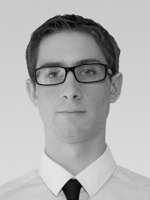
\includegraphics[width=0.5\columnwidth]{../IMG_7936-Modifier_cv}
	\vspace{-0.5cm}
\end{figure}

% Personnal Infos
\begin{flushright}\small
	%Romain \textsc{Reignier} \\
	Avenue Georges Pompidou\\
	Esterel 1 - Appt 119\\
	83160 La Valette du Var\\
	%France\\
	{\footnotesize\href{mailto:romain.reignier@edu.supmeca.fr}{\nolinkurl{romain.reignier@edu.supmeca.fr}}}\\
	06 09 52 16 18\\
	23 ans
\end{flushright}%\normalsize

\begin{flushleft}
% Languages
\SkillSection{Langues}
\SkillItem{Anglais}
Écrit et parlé (TOEIC : 920 pts)\\
\SkillItem{Espagnol}
Niveau Baccalauréat\\
\SkillItem{Allemand}
Débutant
\SmallSep

% Engineering
\SkillSection{Compétences}
Mécanique\\
Conception de systèmes\\
%Analyse des mécanismes\\
Résistance des matériaux\\
%Materials\\
Méthodes numériques\\
Algorithmique\\
%Database\\
%Thermal transferts\\
Automatique\\
Systèmes asservis\\
%Communication\\
Vison par ordinateur\\
Traitement d'images
\SmallSep

% Computer Skills
\SkillSection{Informatique}
\SkillItem{Bureautique}
Word, Excel, PowerPoint, Access, Project, \LaTeX\\
\SkillItem{CAO}
CATIA V5, SolidWorks, ADAMS\\
%\SkillItem{Mathematics}
%Matlab, Maple\\
\SkillItem{Programmation}
\verb!C!/\verb!C++!, Matlab, LabView, Python, Maple, OpenCV, Qt\\
\emph{Embarqué :} Linux, ROS, Arduino, AVR, dsPIC, ARM\\%, assembleur ST8\\
\SkillItem{Développement Web}
HTML5, CSS3, PHP, MySQL\\
\SkillItem{Graphisme}
Photoshop, Lightroom, Illustrator, Gimp, Inkscape\\
% \SkillItem{Others}
% MS Access, MS Project
\SmallSep

% Sports
\SkillSection{Sports}
Cyclisme \& VTT\\
Course à pied\\
%Swimming
%\SmallSep

% Hobbies
\SkillSection{Loisirs}
Photographie\\
Robotique\\
Agriculture\\
Mécanique\\
Brevet d'Initiation à l'Aéronautique
%\SmallSep

% Travels
\SkillSection{Voyages}
Malaisie, Singapour, Togo, Pays-Bas, Allemagne, République Tchèque, Autriche, Suisse
\end{flushleft}
\framebreak


% Right frame
%%%%%%%%%%%%%%%%%%%%
\Huge\bfseries {\color{RoyalBlue} Romain \textsc{Reignier}} \\
\Large\bfseries  Élève ingénieur en mécanique et robotique\\

\normalsize\normalfont

% About me
\begin{AboutMe}
%\emph{Recherche un stage ingénieur de mars 2015 à septembre 2015 en mécatronique.}
\end{AboutMe}

% Formation
\CVSection{Formation}

\CVItem{2013 - aujourd'hui, Université Sud Toulon Var} - \city{La Garde, PACA}\\
Master en Physique et Sciences de l'Ingénieur, spécialité Vision et Commande.\\
Traitement d'image, vision par ordinateur, reconnaissance de formes, trajectographie, détection, estimation.
\SmallSep

\CVItem{2012 - aujourd'hui, SUPMÉCA} - \city{La Garde, PACA}\\
École d'ingénieurs généraliste à dominante mécanique avec parcours Robotique et Systèmes Mécatroniques.
\SmallSep

\CVItem{2009 - 2012, CPGE Victor Hugo} - \city{Caen, Normandie}\\
Physique et Sciences de l'Ingénieur (PSI).\\
Classes préparatoires aux concours d'entrée aux Grandes Écoles.
\SmallSep

\CVItem{2006 - 2009, Lycée Henri Cornat} - \city{Valognes, Normandie}\\
Baccalauréat Scientique, spécialité Physique.
%With Honors.
\Sep

% Experience
\CVSection{Expériences}

\CVItem{Septembre 2013 - Janvier 2014, R\&D CLAAS Tractor} - \city{Vélizy, Yvelines}\\
Stage assistant ingénieur.\\
Travail avec l'expert climatisation sur l'amélioration du système de ventilation de la cabine K07 des tracteurs de fortes puissances.\\
Analyse des résultats d'essais et optimisation des conduits d'air.
\SmallSep

\CVItem{Janvier 2013, DCNS} - \city{Cherbourg, Normandie}\\
Stage opérateur.\\
Travail sur des machines outils à commande numérique pour la création de pièces de sous-marins nucléaires.
\SmallSep

\CVItem{De 2006 à 2012}\\
Divers emplois : Deauville International Polo Club, chantier de l'EPR pour EDF, tourneur-fraiseur, ferme de polyculture-élevage\ldots
\Sep

\CVSection{Projets \& Associations}
\CVItem{Projet de fin d'études} Conception d'un robot mobile pour intervention en zones radioactives en partenariat avec le CEA.
\SmallSep

\CVItem{CRIS}
Club Robotique des élèves Ingénieurs de Supméca : conception, fabrication et programmation de robots mobiles pour participer à la coupe de France de robotique, Eurobot (3 participations).
\SmallSep

\CVItem{Supwave}
Responsable de l'électronique embarquée dans un robot voilier autonome de 4 m.
\SmallSep

\CVItem{Aérocorp}
Responsable de l'électronique et des actionneurs dans un avion d'aéromodélisme.
\SmallSep

\CVItem{Supméca Sans Frontières}
Association humanitaire ayant pour objectif d'assainir l'eau d'un orphelinat togolais.
\SmallSep

\CVItem{Scouts et Guides de France}
8 ans de scoutisme. Chef d'un camp de 30 enfants en 2012 et projet humanitaire au Togo en août 2013.

%\CVSection{Skills}
% \CVItem{Platforms}
%\begin{multicols}{3}
% \begin{compactitem}[\color{RoyalBlue}$\circ$]
% 	\item Lorem 
% 	\item Ipsum 
% \end{compactitem}
%\end{multicols}
%\SmallSep

% \CVItem{Computer software}
% \begin{multicols}{3}
% \begin{compactitem}[\color{RoyalBlue}$\circ$]
% 	\item Lorem 
% 	\item Ipsum 
% 	\item Dolor 
% 	\item Sit 
% 	\item Amet
% 	\item Consectetur 
% 	\item Adipiscing 
% 	\item Elit
% 	\item \ldots
% \end{compactitem}
% \end{multicols}
% \Sep 
% 
% \CVSection{Something other}
% Lorem ipsum dolor sit amet, consectetur adipiscing elit. Vivamus vel bibendum metus. Proin rutrum pharetra molestie. Cras sollicitudin nulla nec leo lobortis in tristique purus pretium. Ut eu felis nulla. Pellentesque condimentum justo ut ligula feugiat nec facilisis tellus ultricies. Nullam sit amet dictum ipsum. Sed lacus neque, hendrerit eu rhoncus nec, pellentesque vitae sem.
% 
% \clearpage
% \framebreak
% \framebreak
% 
% \CVSection{Something else}
% Lorem ipsum dolor sit amet, consectetur adipiscing elit. Vivamus vel bibendum metus. Proin rutrum pharetra molestie. Cras sollicitudin nulla nec leo lobortis in tristique purus pretium. Ut eu felis nulla. Pellentesque condimentum justo ut ligula feugiat nec facilisis tellus ultricies. Nullam sit amet dictum ipsum. Sed lacus neque, hendrerit eu rhoncus nec, pellentesque vitae sem.
% \Sep
% 
% % References
% \CVSection{References}
% References upon request.

%%%%%%%%%%%%%%%%%%%%%%%%%%%%%%%%%%%%%
% End document
%%%%%%%%%%%%%%%%%%%%%%%%%%%%%%%%%%%%%
\end{document}
